% ============================================================
%  J5 — MATIN : MLOps & Industrialisation
%  Julien Rolland — M2 Développement Fullstack
% ============================================================
\documentclass[aspectratio=169, 10pt]{beamer}
% ============================================================
%  PREAMBLE COMMUN — IA, Deep Learning & Machine Learning
%  Julien Rolland — M2 Développement Fullstack
% ============================================================

% --- Langue & encodage ---
\usepackage[utf8]{inputenc}
\usepackage[T1]{fontenc}
\usepackage{babel}
\babelprovide[import, main]{french}

% --- Thème Beamer ---
\usetheme{Madrid}
\usecolortheme{default}

% Palette de bleu académique
\definecolor{jedy_blue}{RGB}{0, 51, 102}       % bleu foncé principal
\definecolor{jedy_mid}{RGB}{0, 102, 179}        % bleu moyen accent
\definecolor{jedy_light}{RGB}{204, 221, 240}    % bleu très clair (fond boxes)
\definecolor{jedy_alert}{RGB}{180, 30, 30}      % rouge pour alertes
\definecolor{jedy_example}{RGB}{0, 120, 60}     % vert pour exemples

% Application des couleurs sur le thème Madrid
\setbeamercolor{palette primary}{bg=jedy_blue, fg=white}
\setbeamercolor{palette secondary}{bg=jedy_mid, fg=white}
\setbeamercolor{palette tertiary}{bg=jedy_blue, fg=white}
\setbeamercolor{palette quaternary}{bg=jedy_blue, fg=white}
\setbeamercolor{structure}{fg=jedy_blue}
\setbeamercolor{frametitle}{bg=jedy_blue, fg=white}
\setbeamercolor{title}{bg=jedy_blue, fg=white}
\setbeamercolor{block title}{bg=jedy_mid, fg=white}
\setbeamercolor{block body}{bg=jedy_light, fg=black}
\setbeamercolor{block title alerted}{bg=jedy_alert, fg=white}
\setbeamercolor{block body alerted}{bg=jedy_light, fg=black}
\setbeamercolor{block title example}{bg=jedy_example, fg=white}
\setbeamercolor{block body example}{bg=jedy_light, fg=black}

% --- Typographie ---
\usepackage{lmodern}
\setbeamerfont{title}{size=\Large, series=\bfseries}
\setbeamerfont{frametitle}{size=\normalsize, series=\bfseries}

% --- Navigation : suppression des icônes de navigation par défaut ---
\setbeamertemplate{navigation symbols}{}

% --- Numérotation des slides ---
\setbeamertemplate{footline}{%
  \leavevmode%
  \hbox{%
    \begin{beamercolorbox}[wd=.333\paperwidth,ht=2.25ex,dp=1ex,center]{author in head/foot}%
      \usebeamerfont{author in head/foot}\insertshortauthor
    \end{beamercolorbox}%
    \begin{beamercolorbox}[wd=.334\paperwidth,ht=2.25ex,dp=1ex,center]{title in head/foot}%
      \usebeamerfont{title in head/foot}\insertshorttitle
    \end{beamercolorbox}%
    \begin{beamercolorbox}[wd=.333\paperwidth,ht=2.25ex,dp=1ex,right]{date in head/foot}%
      \usebeamerfont{date in head/foot}
      \insertframenumber{} / \inserttotalframenumber\hspace*{2ex}
    \end{beamercolorbox}%
  }%
  \vskip0pt%
}

% --- Maths ---
\usepackage{amsmath, amssymb, amsthm}
\usepackage{bm}          % vecteurs en gras : \bm{w}

% --- Code source ---
\usepackage{listings}
\usepackage{xcolor}

\lstdefinestyle{pythonstyle}{
  language=Python,
  basicstyle=\ttfamily\footnotesize,
  keywordstyle=\color{jedy_blue}\bfseries,
  commentstyle=\color{gray}\itshape,
  stringstyle=\color{jedy_example},
  numberstyle=\tiny\color{gray},
  numbers=left,
  numbersep=5pt,
  frame=single,
  framerule=0.4pt,
  rulecolor=\color{jedy_light},
  backgroundcolor=\color{jedy_light!40},
  breaklines=true,
  showstringspaces=false,
  tabsize=4,
}
\lstset{style=pythonstyle}

% Alias pratique pour code inline
\newcommand{\code}[1]{\texttt{\small#1}}

% --- Graphiques ---
\usepackage{graphicx}
\usepackage{tikz}
\usetikzlibrary{arrows.meta, positioning, shapes.geometric, fit, calc}
\usepackage{pgfplots}
\pgfplotsset{compat=1.18}

% --- Tableaux ---
\usepackage{booktabs}
\usepackage{array}

% --- Icônes (optionnel, nécessite fontawesome5) ---
% \usepackage{fontawesome5}

% --- Macros ML/DL courantes ---
\newcommand{\R}{\mathbb{R}}
\newcommand{\E}{\mathbb{E}}
\newcommand{\Loss}{\mathcal{L}}
\newcommand{\dataset}{\mathcal{D}}
\newcommand{\X}{\mathbf{X}}
\newcommand{\y}{\mathbf{y}}
\newcommand{\w}{\mathbf{w}}
\newcommand{\W}{\mathbf{W}}
\newcommand{\grad}{\nabla}
\newcommand{\T}{^{\top}}         % transposée : \X\T
\newcommand{\lr}{\alpha}         % learning rate
\newcommand{\norm}[1]{\left\|#1\right\|}

% Encadré "Objectif pédagogique" en début de section
\newenvironment{objectif}{%
  \begin{alertblock}{Objectif}%
}{%
  \end{alertblock}%
}

% --- Infos du cours (remplacer dans chaque slides.tex) ---
\author[J. Rolland]{Julien Rolland}
\institute[Jedy]{Formation M2 Développement Fullstack}


\title[MLOps]{MLOps \& Industrialisation}
\subtitle{Jour 5 --- Matin}
\date{Jour 5}

% ============================================================
\begin{document}
% ============================================================

\begin{frame}
  \titlepage
\end{frame}

\begin{frame}{Plan du module}
  \tableofcontents
\end{frame}

% ============================================================
\section{Du notebook à la production}
% ============================================================

\begin{frame}{Le fossé R\&D / Production}
  \begin{columns}[T]
    \begin{column}{0.52\textwidth}
      \begin{alertblock}{Le constat}
        «~\textit{It works on my Notebook}~» n'est pas
        une mise en production.\\[4pt]
        \textbf{Contraintes du monde réel :}
        \begin{itemize}
          \item \textbf{Disponibilité :} 1\,000 req/s sans s'effondrer
          \item \textbf{Sécurité :} injection de données corrompues,
                vol de poids du modèle
          \item \textbf{Reproductibilité :} Python 3.10 vs 3.12,
                PyTorch 2.x vs 1.x
        \end{itemize}
      \end{alertblock}
    \end{column}
    \begin{column}{0.44\textwidth}
      \begin{exampleblock}{Le rôle du MLOps}
        Créer un \textbf{pont stable} entre le
        Data Scientist et le DevOps.
        \vspace{4pt}
        \begin{center}
          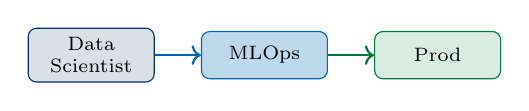
\begin{tikzpicture}[font=\scriptsize,
            blk/.style={draw, rounded corners=3pt, align=center,
                        minimum width=1.6cm, minimum height=0.6cm},
            arr/.style={->, thick}]
            \node[blk, fill=jedy_blue!15, draw=jedy_blue] (ds)
              at (0,0) {Data\\Scientist};
            \node[blk, fill=jedy_mid!25, draw=jedy_mid] (ml)
              at (2.2,0) {MLOps};
            \node[blk, fill=jedy_example!15, draw=jedy_example] (dv)
              at (4.4,0) {Prod};
            \draw[arr, jedy_mid] (ds) -- (ml);
            \draw[arr, jedy_example] (ml) -- (dv);
          \end{tikzpicture}
        \end{center}
      \end{exampleblock}
      \smallskip
      \begin{block}{Au programme}
        Sérialisation \textbullet{} Serving \textbullet{} Docker
        \textbullet{} Monitoring \textbullet{} CI/CD
      \end{block}
    \end{column}
  \end{columns}
\end{frame}

% ============================================================
\section{Sérialiser et optimiser}
% ============================================================

\begin{frame}[fragile]{Sérialisation (1/2) --- le danger de Pickle}
  \begin{columns}[T]
    \begin{column}{0.52\textwidth}
      \begin{block}{Pickle --- le réflexe Python}
\begin{lstlisting}[language=Python]
import pickle

with open("model.pkl", "wb") as f:
    pickle.dump(model, f)

# Charger -- danger si source inconnue !
with open("model.pkl", "rb") as f:
    model = pickle.load(f)
\end{lstlisting}
      \end{block}
      \vspace{2pt}
      \begin{exampleblock}{Avantage}
        Simple, natif, aucune dépendance supplémentaire.
      \end{exampleblock}
    \end{column}
    \begin{column}{0.44\textwidth}
      \begin{alertblock}{Risque de sécurité critique}
        Pickle peut \textbf{exécuter du code arbitraire}
        à la désérialisation.\\[4pt]
        Ne jamais charger un \texttt{.pkl} d'origine inconnue.
      \end{alertblock}
      \smallskip
      \begin{alertblock}{Rigidité = dette technique}
        \begin{itemize}
          \item Nécessite le \textbf{même code source}
                et les mêmes versions de classes
          \item Incompatible entre versions de Python
          \item Inutilisable depuis Java, Go, Rust, etc.
        \end{itemize}
      \end{alertblock}
    \end{column}
  \end{columns}
\end{frame}

\begin{frame}[fragile]{Sérialisation (2/2) --- ONNX \& l'indépendance}
  \begin{columns}[T]
    \begin{column}{0.52\textwidth}
      \begin{exampleblock}{ONNX --- Open Neural Network Exchange}
        Modèle sous forme de \textbf{graphe statique figé} :
        \begin{itemize}
          \item \textbf{Standard universel :} portable partout
          \item \textbf{Vitesse :} souvent plus rapide que PyTorch brut
        \end{itemize}
      \end{exampleblock}
      \vspace{2pt}
\begin{lstlisting}[language=Python]
import torch.onnx
torch.onnx.export(
    model, dummy_input, "model.onnx",
    input_names=["x"], output_names=["y"],
)
import onnxruntime as ort
sess = ort.InferenceSession("model.onnx")
out = sess.run(None, {"x": x_np})
\end{lstlisting}
    \end{column}
    \begin{column}{0.44\textwidth}
      \begin{center}
        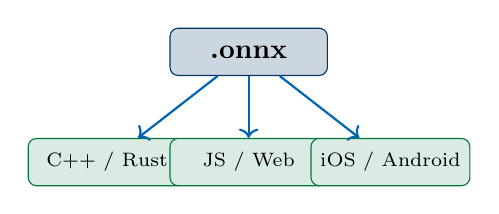
\begin{tikzpicture}[font=\scriptsize,
          blk/.style={draw, rounded corners=3pt, align=center,
                      minimum width=2.0cm, minimum height=0.6cm},
          arr/.style={->, thick, jedy_mid}]
          \node[blk, fill=jedy_blue!20, draw=jedy_blue,
                font=\normalsize\bfseries] (onnx) at (0, 1.4) {.onnx};
          \node[blk, fill=jedy_example!15, draw=jedy_example] (cpp)
            at (-1.8, 0) {C++ / Rust};
          \node[blk, fill=jedy_example!15, draw=jedy_example] (web)
            at (0, 0) {JS / Web};
          \node[blk, fill=jedy_example!15, draw=jedy_example] (mob)
            at (1.8, 0) {iOS / Android};
          \draw[arr] (onnx) -- (cpp);
          \draw[arr] (onnx) -- (web);
          \draw[arr] (onnx) -- (mob);
        \end{tikzpicture}
      \end{center}
      \vspace{4pt}
      \begin{block}{Alternatives PyTorch}
        \begin{itemize}
          \item \texttt{state\_dict} --- poids seuls
          \item \texttt{torch.jit.script} --- TorchScript
          \item \texttt{safetensors} --- sans exécution de code
        \end{itemize}
      \end{block}
    \end{column}
  \end{columns}
\end{frame}

\begin{frame}{L'IA «~On-Edge~» --- zéro serveur, zéro latence}
  \begin{columns}[T]
    \begin{column}{0.52\textwidth}
      \begin{block}{Concept}
        Faire tourner l'IA \textbf{directement chez l'utilisateur} :
        navigateur, mobile, IoT.\\[4pt]
        \textbf{Outils :}
        \begin{itemize}
          \item \textbf{ONNX Runtime Web} --- modèle ONNX dans le navigateur
          \item \textbf{TensorFlow.js} --- JavaScript natif
          \item \textbf{MediaPipe / CoreML} --- vision sur mobile
        \end{itemize}
      \end{block}
    \end{column}
    \begin{column}{0.44\textwidth}
      \begin{exampleblock}{Avantages stratégiques}
        \begin{itemize}
          \item \textbf{Coût :} facture serveur proche de 0€ ---
                le client fournit la puissance de calcul
          \item \textbf{Confidentialité :} la donnée ne quitte
                jamais l'appareil --- RGPD-friendly par design
          \item \textbf{Réactivité :} pas de latence réseau,
                idéal pour la vidéo temps réel
        \end{itemize}
      \end{exampleblock}
      \vspace{2pt}
      \begin{alertblock}{Contrainte}
        Taille limitée par la RAM du device ---
        d'où l'importance de la quantization.
      \end{alertblock}
    \end{column}
  \end{columns}
\end{frame}

\begin{frame}{Optimisation de l'inférence --- «~Speed is a Feature~»}
  \begin{columns}[T]
    \begin{column}{0.31\textwidth}
      \begin{block}{Quantization}
        Passer les poids de \textbf{Float32 à Int8}.
        \begin{itemize}
          \item Gain de vitesse $\times 3$
          \item Poids du modèle $-75\,\%$
          \item Perte de précision $< 1\,\%$
        \end{itemize}
      \end{block}
    \end{column}
    \begin{column}{0.31\textwidth}
      \begin{block}{Pruning}
        Supprimer les connexions dont les poids
        sont proches de zéro.
        \begin{itemize}
          \item Réseau \textbf{creux} (\textit{sparse})
          \item 50--90\,\% des poids supprimables
          \item Fine-tuning nécessaire après
        \end{itemize}
      \end{block}
    \end{column}
    \begin{column}{0.31\textwidth}
      \begin{block}{Compilation Hardware}
        Compiler le graphe pour la carte cible :
        \begin{itemize}
          \item \textbf{TensorRT} --- GPU NVIDIA
          \item \textbf{OpenVINO} --- CPU Intel
          \item \textbf{CoreML} --- Apple Silicon
        \end{itemize}
      \end{block}
    \end{column}
  \end{columns}
  \medskip
  \begin{center}
    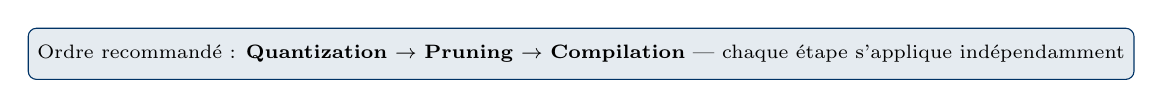
\begin{tikzpicture}[font=\scriptsize]
      \node[draw, rounded corners=3pt, fill=jedy_blue!10, draw=jedy_blue,
            align=center, minimum width=12cm, minimum height=0.65cm]
        {Ordre recommandé :
         \textbf{Quantization} $\to$
         \textbf{Pruning} $\to$
         \textbf{Compilation} ---
         chaque étape s'applique indépendamment};
    \end{tikzpicture}
  \end{center}
\end{frame}

% ============================================================
\section{Serving avec FastAPI}
% ============================================================

\begin{frame}[fragile]{Serving avec FastAPI --- l'architecture Singleton}
  \begin{columns}[T]
    \begin{column}{0.52\textwidth}
      \begin{alertblock}{Anti-pattern à bannir}
        Charger le modèle \textbf{dans} la route API $\to$
        500 Mo rechargés à chaque requête $\to$
        latence + RAM saturée.
      \end{alertblock}
      \vspace{2pt}
\begin{lstlisting}[language=Python]
from contextlib import asynccontextmanager
from fastapi import FastAPI

@asynccontextmanager
async def lifespan(app: FastAPI):
    app.state.model = load_model("model.onnx")
    yield
    app.state.model = None
app = FastAPI(lifespan=lifespan)
@app.post("/predict")
async def predict(data: InputData):
    return app.state.model.run(data)
\end{lstlisting}
    \end{column}
    \begin{column}{0.44\textwidth}
      \begin{exampleblock}{Le pattern Singleton}
        Le modèle est chargé \textbf{une seule fois}
        au démarrage, maintenu en mémoire
        partagée entre toutes les requêtes.
      \end{exampleblock}
      \vspace{2pt}
      \begin{block}{Événements \texttt{lifespan}}
        \begin{itemize}
          \item \textbf{Startup :} charger modèle,
                connexion BDD, warmup GPU
          \item \textbf{Shutdown :} libérer GPU,
                fermer connexions proprement
        \end{itemize}
      \end{block}
    \end{column}
  \end{columns}
\end{frame}

\begin{frame}{FastAPI pour les devs Fullstack}
  \begin{columns}[T]
    \begin{column}{0.46\textwidth}
      \begin{block}{Pydantic --- typage fort}
        Valider automatiquement les entrées JSON :
        \begin{itemize}
          \item Évite les crashs sur données malformées
          \item Erreurs 422 auto-générées avec détail
          \item Intégration native FastAPI
        \end{itemize}
      \end{block}
      \smallskip
      \begin{block}{Asynchronisme}
        \texttt{async def} pour ne pas bloquer
        l'Event Loop pendant les I/O :
        \begin{itemize}
          \item Requêtes BDD, appels HTTP externes
          \item Inférence : déléguer au
                \texttt{ThreadPoolExecutor}
        \end{itemize}
      \end{block}
    \end{column}
    \begin{column}{0.50\textwidth}
      \begin{exampleblock}{Swagger UI automatique}
        Documentation sur \texttt{/docs} ---
        indispensable pour l'intégration Front-end.
        \vspace{4pt}
        \begin{center}
          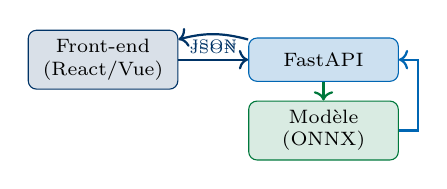
\begin{tikzpicture}[font=\scriptsize,
            blk/.style={draw, rounded corners=3pt, align=center,
                        minimum width=1.9cm, minimum height=0.55cm},
            arr/.style={->, thick}]
            \node[blk, fill=jedy_blue!15, draw=jedy_blue] (front)
              at (0, 0) {Front-end\\(React/Vue)};
            \node[blk, fill=jedy_mid!20, draw=jedy_mid] (api)
              at (2.8, 0) {FastAPI};
            \node[blk, fill=jedy_example!15, draw=jedy_example] (model)
              at (2.8,-0.9) {Modèle\\(ONNX)};
            \draw[arr, jedy_blue] (front) -- node[above, font=\tiny] {JSON} (api);
            \draw[arr, jedy_example] (api) -- (model);
            \draw[arr, jedy_mid] (model) -- ++(1.2,0) |- (api.east);
            \draw[arr, jedy_blue, bend right=15] (api) to
              node[below, font=\tiny] {JSON} (front);
          \end{tikzpicture}
        \end{center}
      \end{exampleblock}
      \smallskip
      \begin{alertblock}{Intérêt terrain}
        Vous connaissez déjà le paradigme REST ---
        FastAPI l'applique à l'IA.
      \end{alertblock}
    \end{column}
  \end{columns}
\end{frame}

\begin{frame}{Le pipeline d'inférence complet}
  \begin{center}
    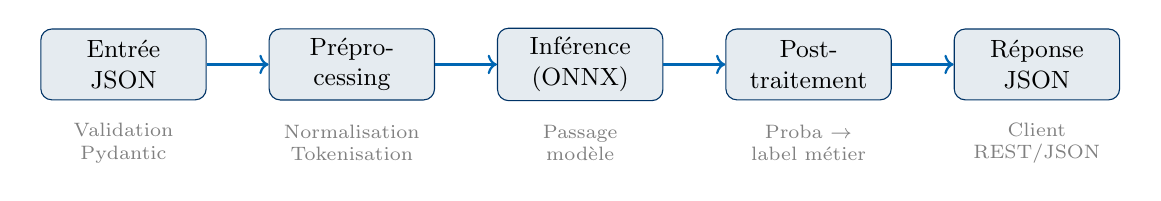
\begin{tikzpicture}[font=\small,
      blk/.style={draw, rounded corners=4pt, align=center,
                  minimum width=2.1cm, minimum height=0.9cm,
                  fill=jedy_blue!10, draw=jedy_blue},
      arr/.style={->, thick, jedy_mid}]
      \node[blk] (in)   at (0,   0) {Entrée\\JSON};
      \node[blk] (pre)  at (2.9, 0) {Prépro-\\cessing};
      \node[blk] (inf)  at (5.8, 0) {Inférence\\(ONNX)};
      \node[blk] (post) at (8.7, 0) {Post-\\traitement};
      \node[blk] (out)  at (11.6,0) {Réponse\\JSON};
      \draw[arr] (in) -- (pre);
      \draw[arr] (pre) -- (inf);
      \draw[arr] (inf) -- (post);
      \draw[arr] (post) -- (out);
      \node[font=\scriptsize, color=gray, text width=2.2cm, align=center]
        at (0,   -1.0) {Validation\\Pydantic};
      \node[font=\scriptsize, color=gray, text width=2.2cm, align=center]
        at (2.9, -1.0) {Normalisation\\Tokenisation};
      \node[font=\scriptsize, color=gray, text width=2.2cm, align=center]
        at (5.8, -1.0) {Passage\\modèle};
      \node[font=\scriptsize, color=gray, text width=2.2cm, align=center]
        at (8.7, -1.0) {Proba $\to$\\label métier};
      \node[font=\scriptsize, color=gray, text width=2.2cm, align=center]
        at (11.6,-1.0) {Client\\REST/JSON};
    \end{tikzpicture}
  \end{center}
  \medskip
  \begin{columns}[T]
    \begin{column}{0.50\textwidth}
      \begin{alertblock}{Point critique : cohérence du prétraitement}
        Le preprocessing doit être \textbf{strictement identique}
        au code d'entraînement --- même scaler, même tokenizer,
        mêmes paramètres.
      \end{alertblock}
    \end{column}
    \begin{column}{0.46\textwidth}
      \begin{exampleblock}{Bonne pratique}
        Empaqueter le prétraitement \textbf{dans} le modèle
        ONNX ou le versionner avec lui
        (ex: \texttt{sklearn Pipeline} sérialisé avec \texttt{safetensors}).
      \end{exampleblock}
    \end{column}
  \end{columns}
\end{frame}

% ============================================================
\section{Docker et CI/CD}
% ============================================================

\begin{frame}{Containerisation avec Docker}
  \begin{columns}[T]
    \begin{column}{0.52\textwidth}
      \begin{block}{Pourquoi Docker en IA ?}
        \begin{itemize}
          \item \textbf{Environnement figé :} Python, CUDA, drivers
                toujours identiques en dev, staging, prod
          \item \textbf{Isolation GPU :} NVIDIA Container Toolkit
          \item \textbf{Reproductibilité :} même image partout
        \end{itemize}
      \end{block}
      \smallskip
      \begin{alertblock}{Le problème du poids}
        Les images Data Science sont lourdes (plusieurs Go) à
        cause de PyTorch et CUDA.\\[2pt]
        Solution : images \textbf{slim} + ne copier que le
        nécessaire.
      \end{alertblock}
    \end{column}
    \begin{column}{0.44\textwidth}
      \begin{exampleblock}{Bonnes pratiques}
        \begin{itemize}
          \item Partir de \texttt{python:3.10-slim}
                (pas \texttt{:latest})
          \item \textbf{Multi-stage build} : compiler dans une
                image lourde, exécuter dans une image légère
          \item Ne jamais commiter des poids ou
                des données dans l'image
          \item Utiliser \texttt{.dockerignore}
        \end{itemize}
      \end{exampleblock}
      \vspace{2pt}
      \begin{block}{GPU en prod}
        \texttt{nvidia/cuda:12.1-base} comme base
        + \texttt{--gpus all} au \texttt{docker run}.
      \end{block}
    \end{column}
  \end{columns}
\end{frame}

\begin{frame}[fragile]{Dockerfile --- optimisation pour l'ingénieur}
  \begin{columns}[T]
    \begin{column}{0.52\textwidth}
\begin{lstlisting}[language=bash]
FROM python:3.10-slim AS base
WORKDIR /app

# Layer caching : deps avant le code
COPY requirements.txt .
RUN pip install --no-cache-dir -r requirements.txt

# Code source (invalide le cache si change)
COPY src/ ./src/

# Securite : pas de root en prod
RUN useradd --no-create-home appuser
USER appuser

EXPOSE 8000
CMD ["uvicorn", "src.main:app", "--host", "0.0.0.0"]
\end{lstlisting}
    \end{column}
    \begin{column}{0.44\textwidth}
      \begin{exampleblock}{Layer caching}
        Les dépendances changent rarement : les installer
        \textbf{avant} de copier le code.\\[2pt]
        Docker réutilise le cache si
        \texttt{requirements.txt} n'a pas changé ---
        rebuild quasi instantané.
      \end{exampleblock}
      \vspace{2pt}
      \begin{alertblock}{Sécurité : non-root}
        Ne jamais lancer l'API en \texttt{root}. Un
        \texttt{useradd} + \texttt{USER} réduit
        drastiquement la surface d'attaque.
      \end{alertblock}
    \end{column}
  \end{columns}
\end{frame}

\begin{frame}{Monitoring \& Dérives (\textit{Drift})}
  \begin{columns}[T]
    \begin{column}{0.52\textwidth}
      \begin{alertblock}{Pourquoi mon modèle «~meurt~» en prod ?}
        \begin{itemize}
          \item \textbf{Data Drift :} les données changent
                (ex: nouvel argot sur les réseaux sociaux)
          \item \textbf{Concept Drift :} le monde change
                (ex: prédictions avant/après une crise)
          \item \textbf{Infrastructure :} mise à jour de dépendance,
                changement de format d'entrée
        \end{itemize}
      \end{alertblock}
    \end{column}
    \begin{column}{0.44\textwidth}
      \begin{exampleblock}{Pipeline de surveillance}
        \begin{enumerate}
          \item \textbf{Logger} les prédictions en production
          \item \textbf{Collecter} la vérité terrain
          \item \textbf{Comparer} distributions et métriques
          \item \textbf{Alerter} si dégradation $>$ seuil
          \item \textbf{Ré-entraîner} sur les nouvelles données
        \end{enumerate}
      \end{exampleblock}
      \vspace{2pt}
      \begin{block}{Outils}
        \textbf{Evidently} \textbullet{} \textbf{WhyLogs}
        \textbullet{} \textbf{MLflow} \textbullet{} \textbf{Grafana}
      \end{block}
    \end{column}
  \end{columns}
\end{frame}

\begin{frame}{Conclusion --- CI/CD pour le ML}
  \begin{columns}[T]
    \begin{column}{0.52\textwidth}
      \begin{block}{Automatisation : CI/CD ML}
        \begin{itemize}
          \item \textbf{Tests unitaires :} preprocessing,
                postprocessing
          \item \textbf{Tests modèle :} accuracy $>$ seuil minimal
                sur un jeu de validation figé
          \item \textbf{Build \& push} de l'image Docker
          \item \textbf{Déploiement :} staging puis prod
        \end{itemize}
      \end{block}
      \smallskip
      \begin{exampleblock}{Stratégies de déploiement}
        \begin{itemize}
          \item \textbf{Canary :} 5\,\% du trafic
                sur le nouveau modèle
          \item \textbf{A/B Testing :} comparaison contrôlée
          \item \textbf{Shadow mode :} logs sans impact client
        \end{itemize}
      \end{exampleblock}
    \end{column}
    \begin{column}{0.44\textwidth}
      \begin{alertblock}{Ce que vous avez appris}
        \begin{itemize}
          \item Sérialiser avec ONNX pour la portabilité
          \item Servir avec FastAPI (pattern Singleton)
          \item Conteneuriser avec Docker (non-root,
                layer caching)
          \item Surveiller les dérives en production
        \end{itemize}
      \end{alertblock}
      \smallskip
      \begin{exampleblock}{Place au Challenge !}
        \textbf{Vous avez le moteur, vous avez la boîte} ---
        maintenant mettez votre modèle en production.
      \end{exampleblock}
    \end{column}
  \end{columns}
\end{frame}

\end{document}
